\documentclass[UTF8,fontset=none,11pt]{ctexart}

% ---------- 基础宏包 ----------
\usepackage[a4paper,margin=2.2cm]{geometry}
\usepackage{amsmath,amssymb}
\usepackage{enumitem}
\usepackage{xcolor}
\usepackage{booktabs}
\usepackage{array}
\usepackage{longtable}
\usepackage{tikz}
\usepackage{hyperref}
\usetikzlibrary{positioning,arrows.meta,shapes.geometric,fit,backgrounds,automata,calc}

\setCJKmainfont{PingFang SC}
\setCJKsansfont{PingFang SC}
\setCJKmonofont{PingFang SC}

% ---------- 颜色 ----------
\definecolor{maincol}{RGB}{30,90,160}
\definecolor{accent}{RGB}{200,80,30}
\definecolor{softbg}{RGB}{243,247,252}
\definecolor{defbg}{RGB}{238,246,240}
\definecolor{defrule}{RGB}{60,140,90}
\definecolor{warnbg}{RGB}{253,245,233}
\definecolor{warnrule}{RGB}{200,140,40}

% ---------- 超链接 ----------
\hypersetup{colorlinks=true,linkcolor=maincol,urlcolor=accent,
  pdftitle={词法分析 NFA 与 DFA 笔记},pdfauthor={Summary}}

% ---------- 列表风格 ----------
\setlist[itemize]{leftmargin=1.4em,itemsep=2pt,topsep=2pt}
\setlist[enumerate]{leftmargin=1.6em,itemsep=2pt,topsep=2pt}

% ---------- 自定义可分页标注盒子（不依赖 tcolorbox） ----------
\newenvironment{defbox}[1][]{%
  \par\medskip\noindent{\color{defrule}\rule{\linewidth}{1.1pt}}\par\nopagebreak
  \noindent{\bfseries\color{defrule}#1}\par\nopagebreak\smallskip}%
  {\par\nopagebreak\smallskip\noindent{\color{defrule}\rule{\linewidth}{0.4pt}}\par\medskip}

\newenvironment{notebox}[1][]{%
  \par\medskip\noindent{\color{maincol}\rule{\linewidth}{1.1pt}}\par\nopagebreak
  \noindent{\bfseries\color{maincol}#1}\par\nopagebreak\smallskip}%
  {\par\nopagebreak\smallskip\noindent{\color{maincol}\rule{\linewidth}{0.4pt}}\par\medskip}

\newenvironment{warnbox}[1][]{%
  \par\medskip\noindent{\color{warnrule}\rule{\linewidth}{1.1pt}}\par\nopagebreak
  \noindent{\bfseries\color{warnrule}#1}\par\nopagebreak\smallskip}%
  {\par\nopagebreak\smallskip\noindent{\color{warnrule}\rule{\linewidth}{0.4pt}}\par\medskip}

% 页码引用标记
\newcommand{\pg}[1]{{\small\color{gray}\,[p#1]}}
% 中英术语
\newcommand{\term}[2]{\textbf{#1}（#2）}

\title{\bfseries 编译原理 · 词法分析（二）：有穷自动机 NFA 与 DFA\\[2pt]
\large Lexical Analysis: NFA \& DFA —— 详细学习笔记}
\author{基于课件 \texttt{2.Lexical Analysis\_NFA\_DFA.pdf}（中山大学 · 赵帅）整理}
\date{}

\begin{document}
\maketitle
\thispagestyle{empty}

\begin{notebox}[本笔记说明]
本笔记完整覆盖第 2 讲《词法分析：NFA 与 DFA》共 80 页。它承接第 1 讲——上一讲学会了用
\textbf{正则表达式（Regular Expression, RE）}\emph{描述}单词的模式（这是"规范"），
本讲解决\emph{如何把规范变成能真正运行的识别器}（这是"实现"）。
主线是一条清晰的"流水线"：
\[
\text{RE}\xrightarrow{\text{Thompson}}\text{NFA}\xrightarrow{\text{子集构造}}\text{DFA}
\xrightarrow{\text{最小化}}\text{最小 DFA}\to\text{表驱动实现}\to\text{词法分析器}.
\]
每个知识点用 \pg{页码} 标注来源；专业术语首次出现给出\textbf{中文（English）}对照与通俗解释。
\end{notebox}

\tableofcontents
\vspace{4pt}\hrule

% ============================================================
\section{全局蓝图：从规范到实现（第 1--2 页）}
% ============================================================
本讲处在"从规范到实现（From Specification to Implementation）"这张大地图的\textbf{右半部分} \pg{1,2}。
请先记住这条主链路——后面每一节都是在讲它的某一段：

\begin{center}
\begin{tikzpicture}[font=\small,
  n/.style={draw,rounded corners=2pt,fill=softbg,minimum height=0.72cm,align=center,inner sep=3pt},
  hi/.style={draw,rounded corners=2pt,fill=defbg,minimum height=0.72cm,align=center,inner sep=3pt},
  arr/.style={-{Latex[length=2mm]},thick}]
\node[n] (re) {正则表达式\\RE（规范）};
\node[hi,right=1.5cm of re] (nfa) {NFA};
\node[hi,right=1.5cm of nfa] (dfa) {DFA};
\node[hi,below=1.0cm of dfa] (min) {最小 DFA\\Minimal DFA};
\node[n,left=1.5cm of min] (tab) {表驱动\\Table-Driven};
\node[n,left=1.5cm of tab] (lex) {词法分析器\\（实现）};
\draw[arr] (re) -- node[above,font=\footnotesize]{Thompson} (nfa);
\draw[arr] (nfa) -- node[above,font=\footnotesize]{子集构造} (dfa);
\draw[arr] (dfa) -- node[right,font=\footnotesize]{最小化} (min);
\draw[arr] (min) -- node[above,font=\footnotesize]{生成表} (tab);
\draw[arr] (tab) -- node[above,font=\footnotesize]{模拟运行} (lex);
\end{tikzpicture}
\end{center}

\begin{notebox}[四步走（本讲的四个核心算法）\pg{13}]
① \textbf{RE $\to$ NFA}：Thompson 算法（Thompson Algorithm）。\quad
② \textbf{NFA $\to$ DFA}：子集构造法（Subset-Construction Algorithm）。\\
③ \textbf{DFA 最小化}：分割法（Partition Algorithm）。\quad
④ \textbf{DFA $\to$ 表驱动实现}（Table-Driven Implementation）。
\end{notebox}

% ============================================================
\section{有穷自动机基础（第 3--13 页）}
% ============================================================

\subsection{为什么需要有穷自动机 \pg{3,4}}
\begin{defbox}[有穷自动机（Finite Automata, FA）\pg{3,4}]
\textbf{RE 只是语言的"规范（specification）"}——它只定义了"哪些串属于这个语言"，本身不会"跑"。
要真正\textbf{识别}串，需要一个\emph{实现}：\textbf{有穷自动机}。\\
\textbf{自动机（automaton，复数 automata）}=一台机器/一段程序；\textbf{有穷自动机}=
\emph{状态数量有限}的程序。它很像\textbf{转换图（transition diagram）}：有\textbf{状态}和\textbf{带标号的边}，
有\emph{唯一}的开始状态、\emph{一个或多个}接受状态。
\end{defbox}

\begin{notebox}[一句话对应关系 \pg{4}]
\textbf{正则表达式 = 规范（要识别什么）}；\textbf{有穷自动机 = 实现（怎么识别）}。
两类自动机：\term{非确定有穷自动机}{NFA, Nondeterministic Finite Automata} 与
\term{确定有穷自动机}{DFA, Deterministic Finite Automata}。
\end{notebox}

\subsection{转换图：FA 的画法 \pg{5}}
\begin{defbox}[转换图的两类要素 \pg{5}]
\textbf{节点（Node）= 状态（state）}：每个状态代表识别过程中"可能出现的一种情形"。
\begin{itemize}
  \item \textbf{初始态（Start）}：\emph{唯一}，用一个标着 \texttt{start} 的箭头指向它。
  \item \textbf{接受态 / 终态（Final / Accepting）}：\emph{可有多个}，用\textbf{双圈}表示。
\end{itemize}
\textbf{边（Edge）= 转移（transition）}：\emph{有向}，标注输入符号；表示"读到该符号时从一个状态走到另一个状态"。
\end{defbox}

\begin{center}
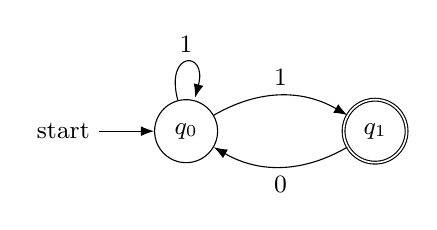
\begin{tikzpicture}[font=\small,>=Latex,node distance=2.0cm,on grid,
  st/.style={circle,draw,minimum size=0.8cm},
  acc/.style={circle,draw,double,minimum size=0.8cm}]
\node[st] (s0) {$q_0$};
\node[acc,right=2.4cm of s0] (s1) {$q_1$};
\draw[<-] (s0) -- ++(-1.1,0) node[left]{start};
\draw[->] (s0) to[bend left] node[above]{1} (s1);
\draw[->] (s1) to[bend left] node[below]{0} (s0);
\draw[->] (s0) edge[loop above] node{1} (s0);
\end{tikzpicture}
\\[2pt]
{\footnotesize 单圈=普通态，双圈=接受态，\texttt{start} 箭头指开始态。}
\end{center}

\subsection{FA 就是"语言识别程序" \pg{6,7}}
\begin{defbox}[FA 的语言（Language of FA）\pg{6}]
FA 是一个给字符串\textbf{分类}的程序，输出 \textbf{接受（accept）}或\textbf{拒绝（reject）}，
也就是\emph{识别一门语言}的程序。\\
对给定串 $x$：若存在一条转移序列把它从\textbf{开始态}带到某个\textbf{接受态}，则称 $x$ \textbf{被该 FA 接受}，否则\textbf{拒绝}。\\
\textbf{$L(\text{FA})$ = 被该 FA 接受的所有串的集合}；并且有 $\boxed{L(\text{FA})\equiv L(\text{RE})}$——FA 与 RE 描述能力相同。
\end{defbox}

\begin{notebox}[小例子 \pg{7}]
上图（$\Sigma=\{0,1\}$）识别的语言是\textbf{"任意多个 1 之后跟恰好一个 0"}。
判定：\texttt{0}\,√、\texttt{1}\,×、\texttt{11110}\,√、\texttt{11101}\,×、\texttt{11100}\,×、\texttt{1111110}\,√。
\end{notebox}

\subsection{DFA 与 NFA 的区别 \pg{8}}
\begin{defbox}[DFA vs.\ NFA \pg{8}]
\textbf{确定有穷自动机（DFA）}：任一时刻\emph{只}处于\textbf{一个}状态。
\begin{itemize}
  \item 每个状态对每个输入符号\textbf{恰有一个}转移；\textbf{没有 $\varepsilon$ 转移（no $\varepsilon$-moves）}；在状态图中\textbf{只走一条路径}。
\end{itemize}
\textbf{非确定有穷自动机（NFA）}：可\emph{同时}处于\textbf{多个}状态。
\begin{itemize}
  \item 一个状态对同一输入可有\textbf{多个}转移；\textbf{允许 $\varepsilon$ 转移}（不读输入就能跳转）；可"选择"走哪条路。
  \item \textbf{接受规则}：只要\emph{存在某一条}路径在输入结束时停在接受态，NFA 就\textbf{接受}。
\end{itemize}
\end{defbox}

\begin{notebox}[NFA 的"非确定"怎么理解]
把 NFA 想成"\textbf{可以同时分身走所有岔路}"：只要有\emph{任意一个分身}最终落在接受态，整串就算被接受。
而 DFA 像"\textbf{一条道走到黑}"：每一步路线唯一，毫无悬念。
\end{notebox}

\subsection{FA 的形式定义：五元组 \pg{9}}
\begin{defbox}[FA 的五元组 $(\Sigma,S,n,F,\delta)$ \pg{9}]
\begin{itemize}
  \item $\Sigma$：\textbf{输入字母表}（input alphabet）。
  \item $S$：\textbf{状态集}（set of states）。
  \item $n\in S$：\textbf{开始态}（start state）。
  \item $F\subseteq S$：\textbf{接受态集}（accepting states）。
  \item $\delta$：\textbf{转移函数}（transitions），形如 $\delta: S\times \text{Input}\to S$（NFA 中结果是状态\emph{集合}）。
\end{itemize}
\end{defbox}

\subsection{NFA 与 DFA 接受同一串的对比 \pg{10,11}}
以 $(a\,|\,b)^*abb$、输入 \texttt{aabb} 为例：
\begin{itemize}
  \item \textbf{NFA \pg{10}}：有多条可能走法。只需\emph{找到一条}成功序列即可接受：
  $0\xrightarrow{a}0\xrightarrow{a}1\xrightarrow{b}2\xrightarrow{b}3$（终点 3 是接受态）。
  也存在失败序列（一直停在 0），但\textbf{有一条成功即接受}。
  \item \textbf{DFA \pg{11}}：走法\emph{唯一}：
  $0\xrightarrow{a}1\xrightarrow{a}1\xrightarrow{b}2\xrightarrow{b}3$，要么到接受态、要么被拒。
\end{itemize}

\subsection{转换表：FA 的另一种表示 \pg{12,13}}
\begin{defbox}[转换表（Transition Table）\pg{12}]
把 FA 的转移写成一张表：行=状态，列=输入符号，格子=转移到的状态。
\begin{itemize}
  \item \textbf{优点}：能\emph{快速查到}"某状态在某输入下转去哪"。
  \item \textbf{缺点}：\emph{占空间}——字母表大时，多数状态对多数符号都没有转移，表却仍要留位。
  \item \textbf{空间需求}：$O(|S|\times|\Sigma|)$（状态数 $\times$ 字母表大小）。
\end{itemize}
\end{defbox}

% ============================================================
\section{Thompson 算法：RE $\to$ NFA（第 14--22 页）}
% ============================================================
\begin{defbox}[Thompson 构造法（Thompson Algorithm）\pg{14,15}]
一种把\textbf{任意正则表达式}\emph{系统地}转换为 NFA 的方法。核心思想是\textbf{递归}：
先给\emph{原子 RE}造小 NFA，再用三条\emph{归纳规则}把小 NFA 像积木一样\textbf{拼接}成大 NFA。
拼出的 NFA 总是\emph{恰有一个开始态、一个接受态}。
\end{defbox}

\subsection{基础：原子 RE 的 NFA \pg{14}}
\begin{itemize}
  \item \textbf{$\varepsilon$ 的 NFA}：开始态经一条标 $\varepsilon$ 的边直接到接受态（不读字符即可接受空串）。
  \item \textbf{单字符 $a$ 的 NFA}：开始态经一条标 $a$ 的边到接受态（只接受单字符串 \texttt{a}）。
\end{itemize}

\begin{center}
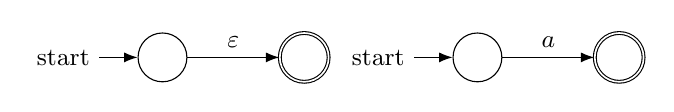
\begin{tikzpicture}[font=\small,>=Latex,node distance=2.2cm,on grid,
  st/.style={circle,draw,minimum size=0.62cm},
  acc/.style={circle,draw,double,minimum size=0.62cm}]
\node[st] (a0) {}; \node[acc,right=1.8cm of a0] (a1) {};
\draw[<-] (a0) -- ++(-0.8,0) node[left]{start};
\draw[->] (a0) -- node[above]{$\varepsilon$} (a1);
\node[st,right=4.0cm of a0] (b0) {}; \node[acc,right=1.8cm of b0] (b1) {};
\draw[<-] (b0) -- ++(-0.8,0) node[left]{start};
\draw[->] (b0) -- node[above]{$a$} (b1);
\end{tikzpicture}
\\[2pt]{\footnotesize 左：$\varepsilon$ 的 NFA；右：单字符 $a$ 的 NFA。}
\end{center}

\subsection{归纳：三条复合规则 \pg{15}}
设 RE $A,B$ 已各自造好 NFA（每个都有唯一 start 和唯一 accept）：

\begin{defbox}[三条拼接规则 \pg{15}]
\begin{enumerate}
  \item \textbf{选择 $R=A\,|\,B$}：新建开始态，用 $\varepsilon$ 边分别进入 $A$、$B$ 的开始态；
  $A$、$B$ 的接受态各用 $\varepsilon$ 边汇入新建的接受态。（"\emph{二选一}"）
  \item \textbf{连接 $R=AB$}：把 $A$ 的接受态用 $\varepsilon$ 边接到 $B$ 的开始态；
  整体开始态取 $A$ 的、接受态取 $B$ 的。（"\emph{先 A 后 B}"）
  \item \textbf{闭包 $R=A^{*}$}：新建开始态，$\varepsilon$ 边既指向 $A$ 的开始态、也\emph{直达}新接受态（对应"零次"）；
  $A$ 的接受态用 $\varepsilon$ 边\emph{回到} $A$ 的开始态（对应"多次"）并指向新接受态。
\end{enumerate}
\end{defbox}

\begin{center}
\begin{tikzpicture}[font=\footnotesize,>=Latex,on grid,
  st/.style={circle,draw,minimum size=0.52cm,inner sep=0pt},
  acc/.style={circle,draw,double,minimum size=0.52cm,inner sep=0pt},
  bx/.style={draw,rounded corners,minimum width=1.0cm,minimum height=0.6cm}]
% A|B
\node[st] (s) {};
\node[bx,above right=0.7cm and 1.3cm of s] (A) {$A$};
\node[bx,below right=0.7cm and 1.3cm of s] (B) {$B$};
\node[acc,below right=0.7cm and 1.3cm of A] (f) {};
\draw[<-] (s) -- ++(-0.7,0);
\draw[->] (s) -- node[above left,inner sep=1pt]{$\varepsilon$} (A);
\draw[->] (s) -- node[below left,inner sep=1pt]{$\varepsilon$} (B);
\draw[->] (A) -- node[above right,inner sep=1pt]{$\varepsilon$} (f);
\draw[->] (B) -- node[below right,inner sep=1pt]{$\varepsilon$} (f);
\node[below=1.4cm of s,font=\small\bfseries] {$R=A\,|\,B$（选择）};
\end{tikzpicture}
\hspace{0.6cm}
\begin{tikzpicture}[font=\footnotesize,>=Latex,on grid,
  bx/.style={draw,rounded corners,minimum width=1.0cm,minimum height=0.6cm}]
\node[bx] (A) {$A$};
\node[bx,right=1.6cm of A] (B) {$B$};
\draw[<-] (A) -- ++(-0.7,0);
\draw[->] (A) -- node[above]{$\varepsilon$} (B);
\draw[->] (B) -- ++(0.7,0);
\node[below=1.0cm of $(A)!0.5!(B)$,font=\small\bfseries] {$R=AB$（连接）};
\end{tikzpicture}
\hspace{0.6cm}
\begin{tikzpicture}[font=\footnotesize,>=Latex,on grid,
  st/.style={circle,draw,minimum size=0.52cm,inner sep=0pt},
  acc/.style={circle,draw,double,minimum size=0.52cm,inner sep=0pt},
  bx/.style={draw,rounded corners,minimum width=1.0cm,minimum height=0.6cm}]
\node[st] (s) {};
\node[bx,right=1.4cm of s] (A) {$A$};
\node[acc,right=1.4cm of A] (f) {};
\draw[<-] (s) -- ++(-0.7,0);
\draw[->] (s) -- node[above]{$\varepsilon$} (A);
\draw[->] (A) -- node[above]{$\varepsilon$} (f);
\draw[->] (A) to[bend left=55] node[above]{$\varepsilon$} (s);
\draw[->] (s) to[bend right=70] node[below]{$\varepsilon$} (f);
\node[below=1.4cm of A,font=\small\bfseries] {$R=A^{*}$（闭包）};
\end{tikzpicture}
\end{center}

\begin{notebox}[例子：$(a\,|\,b)^*abb$ \pg{16,17}]
分步搭积木：先造原子 \texttt{a}、\texttt{b} 的 NFA $\to$ 用规则①得 $(a|b)$ $\to$ 用规则③得 $(a|b)^*$
$\to$ 用规则②把 $(a|b)^*$ 与 \texttt{a}、\texttt{b}、\texttt{b} 依次连接，得到 $(a|b)^*abb$ 的完整 NFA。
\end{notebox}

\subsection{回顾：规范与实现如何衔接 \pg{18--22}}
\begin{itemize}
  \item \textbf{描述链（Revisit）\pg{18}}：语言规范 $\to$ 定义 \textbf{Token} $\to$ Token 的抽象是\textbf{模式（Pattern）}
  $\to$ 模式由 \textbf{RE} 指定（Specify）；\textbf{词素（Lexeme）}是 Token 的\emph{实例（Instance）}、由模式\textbf{匹配（Match）}得到。
  \item \textbf{复合 RE 例子 \pg{20}}：$(ab)^*$、$(a|b)^*$、$(a^*b^*)^*$。
  \item \textbf{消歧（Removing Ambiguity）\pg{20}}：关键字优先（keyword first）、最长匹配（maximal match）、先列者优先（the one listed first）。
  \item \textbf{实现 = 有穷自动机 \pg{20}}：NFA / DFA / 转换表；\textbf{Thompson 算法}把小 NFA 系统地连接成大 NFA。
\end{itemize}

% ============================================================
\section{子集构造法：NFA $\to$ DFA（第 22--31 页）}
% ============================================================

\subsection{为什么要转成 DFA \pg{22,23}}
\begin{defbox}[等价定理 $L(\text{NFA})\equiv L(\text{DFA})$ \pg{23}]
NFA 与 DFA \textbf{描述能力相同}：二者都识别\textbf{正则语言}；对每个 NFA $M$，都\emph{存在}一个 DFA $M'$ 使 $L(M)=L(M')$。
\end{defbox}

\begin{notebox}[各有取舍 \pg{23}]
\textbf{DFA 更费内存}（转移表可能更大），但\textbf{执行更快}：DFA 的转移次数 $=$ 输入长度；NFA 潜在转移数更多。
所以实践中常做 \textbf{NFA $\to$ DFA} 转换——\emph{DFA 的速度优势远超它多占的内存}。
\end{notebox}

\subsection{核心思想与两个待解决问题 \pg{24,25}}
\begin{defbox}[子集构造法（Subset Construction）\pg{24}]
\textbf{DFA 的每一个状态，对应 NFA 的一个状态\emph{集合}}。\\
直觉：读完输入 $a_1a_2\cdots a_n$ 后，DFA 所处的那个状态，正好对应"NFA 从开始态出发、
沿 $a_1a_2\cdots a_n$ 能到达的所有 NFA 状态的集合"。这样就把 NFA 的"同时在多个状态"用 DFA 的"一个集合状态"模拟掉。
\end{defbox}

要把 NFA 变 DFA，必须消除两种"非确定性" \pg{25}：
\begin{enumerate}
  \item 消除 \textbf{$\varepsilon$ 转移}；\quad 2. 消除\textbf{同一状态对同一字符的多个转移}。
\end{enumerate}

\subsection{两个关键运算：$\varepsilon$-closure 与 move \pg{25,26}}
\begin{defbox}[$\varepsilon$-闭包（$\varepsilon$-closure）\pg{25,26}]
\textbf{$\varepsilon\text{-closure}(s)$}：从状态 $s$ 出发，经过\emph{零次或多次} $\varepsilon$ 转移能到达的\textbf{所有状态}的集合。\\
\textbf{$\varepsilon\text{-closure}(T)$}：把集合 $T$ 里\emph{每个}状态的 $\varepsilon$-闭包并起来。\\
\emph{通俗讲}：站在某些状态上，"免费"（不读字符）能溜达到的所有地方，连同自己。
例：若 $s$ 经 $\varepsilon$ 可达 $s_1,s_2$，则 $\varepsilon\text{-closure}(\{s\})=\{s,s_1,s_2\}$。
\end{defbox}

\begin{defbox}[move 运算 \pg{26}]
$\text{move}(T,a)=\{\,t \mid \exists\, s\in T,\ s\xrightarrow{a}t\,\}$：
从集合 $T$ 中\emph{某个}状态出发、读\textbf{一个字符 $a$} 能直接到达的 NFA 状态集合。\\
组合记号：$I_a=\varepsilon\text{-closure}\big(\text{move}(I,a)\big)$——\emph{先走一个 $a$，再做 $\varepsilon$-闭包}，
这正是 DFA 中"集合状态 $I$ 读 $a$ 之后到达的新集合状态"。
\end{defbox}

\subsection{完整算法（三步）\pg{27--30}}
\begin{enumerate}
  \item \textbf{Step 1} 起点：$I=\varepsilon\text{-closure}(\text{开始态})$，作为 DFA 的第一个状态。
  \item \textbf{Step 2} 迭代：对每个尚未处理的集合状态 $I$、每个字符 $x\in\Sigma$，
  求 $I_x=\varepsilon\text{-closure}(\text{move}(I,x))$；遇到\emph{新}集合就登记为新 DFA 状态，直到\textbf{不再产生新集合}。
  \item \textbf{Step 3} 标记接受态：凡\emph{包含原 NFA 任一接受态}的集合状态，标记为 DFA 的接受态。
\end{enumerate}

\begin{notebox}[贯穿例子的转移表 \pg{27--31}]
以一个 NFA（开始态 0，$0\xrightarrow{\varepsilon}1$、$0\xrightarrow{\varepsilon}3$、$1\xrightarrow{a}2$、$3\xrightarrow{b}4$，4 为接受态）为例。
按算法逐步求出下表（$I_a,I_b$ 列即转移目标）：
\end{notebox}

\begin{center}
\begin{longtable}{c l l l c}
\toprule
\textbf{DFA 状态} & \textbf{集合 $I$} & \textbf{$I_a$（读 a）} & \textbf{$I_b$（读 b）} & \textbf{接受?} \\
\midrule
\endhead
$T_0$ & $\{0,1,3\}$ & $\{2,4\}=T_1$ & $\{4\}=T_2$ & 否 \\
$T_1$ & $\{2,4\}$ & $\{\}$（死状态 dead） & $\{1,3\}=T_3$ & \textbf{是} \\
$T_2$ & $\{4\}$ & $\{\}$ & $\{\}$ & \textbf{是} \\
$T_3$ & $\{1,3\}$ & $\{2,4\}=T_1$ & $\{4\}=T_2$ & 否 \\
\bottomrule
\end{longtable}
\end{center}

\begin{warnbox}[易错点：死状态（dead state）\pg{29}]
$\text{move}(\{2,4\},a)=\{\}$（空集），意味着读到 \texttt{a} 后\emph{无路可走}——这对应一个\textbf{死状态}（陷阱状态）。
在严格的 DFA 里，所有"无定义的转移"都指向这个死状态；它\emph{不是接受态}，进去就出不来、整串被拒。
（教材 3.8.3）
\end{warnbox}

% ============================================================
\section{DFA 最小化：分割法（第 32--40 页）}
% ============================================================

\subsection{为什么能最小化、目标是什么 \pg{33}}
\begin{defbox}[最小 DFA 的唯一性 \pg{33}]
对任意给定 DFA，都\emph{存在}一个识别\textbf{相同语言}、状态数\textbf{最少}的等价 DFA，
而且这个\textbf{最小 DFA 是唯一的}（在状态重命名意义下）。
\end{defbox}

\begin{defbox}[等价状态（Equivalent States）\pg{33}]
两个状态 $s,t$ \textbf{等价}，当且仅当同时满足：
\begin{enumerate}
  \item $s,t$ \textbf{要么都是接受态、要么都是非接受态}（同类）；
  \item 对\emph{每个}字符 $x\in\Sigma$，$s$ 与 $t$ 在 $x$ 上转移到的状态\textbf{也是等价}的。
\end{enumerate}
\emph{通俗讲}：两个状态等价 = "\textbf{无论后面再输入什么串，都无法区分它们}"（要么都接受、要么都拒）。
\end{defbox}

\subsection{分割算法（Partition Algorithm）\pg{34}}
\begin{enumerate}
  \item \textbf{初始}：把所有状态分成两组——$\{$接受态$\}$ 和 $\{$非接受态$\}$。
  \item \textbf{细分}：对每个组、每个字符 $x$，看组内各状态在 $x$ 上是否转移到\emph{同一组}；
  若不一致，就把这个组\textbf{拆开}。
  \item \textbf{重复}直到\emph{没有任何组再能被拆分}；每个最终组合并成最小 DFA 的一个状态。
\end{enumerate}

\begin{notebox}[简单例子 \pg{35}]
初始 $\{A\}$（非接受）、$\{BC,AC\}$（接受）。检查 $\{BC,AC\}$：
\texttt{BC} 与 \texttt{AC} 在 \texttt{0} 上都到 \texttt{AC}、在 \texttt{1} 上都到 \texttt{BC}——\emph{任何串都无法区分}，故不拆。
最终 $\{A\}$、$\{BCAC\}$。
\end{notebox}

\begin{notebox}[复杂例子 $\{S,A,B,C,D,E,F\}$ 的分割过程 \pg{36--39}]
\begin{enumerate}
  \item \textbf{初始}：$\{S,A,B\}$（非接受）、$\{C,D,E,F\}$（接受）。
  \item 检查 $\{C,D,E,F\}$：对 \texttt{a}、\texttt{b} 转移都落在 $\{C,D,E,F\}$ 内部，\textbf{全等价，不拆}。
  \item 检查 $\{S,A,B\}$：读 \texttt{a} 时 $S\!\to\!A,\ B\!\to\!A$ 但 $A\!\to\!C$（去了另一组）$\Rightarrow$ \texttt{A} 与 $\{S,B\}$ 不等价，拆出 $\{A\}$。
  \item 再检查 $\{S,B\}$：读 \texttt{b} 时 $S\!\to\!B,\ B\!\to\!\{C,\dots\}$ 不一致 $\Rightarrow$ 拆成 $\{S\}$、$\{B\}$。
  \item \textbf{最终}：$\{C,D,E,F\}$、$\{S\}$、$\{A\}$、$\{B\}$——把 $\{C,D,E,F\}$ 记作一个状态 $C$，画出最小 DFA。
\end{enumerate}
\end{notebox}

\begin{notebox}[练习：判断是否已最小 \pg{40}]
DFA（态 0,1,2,3）：初始 $\{0,3\}$、$\{1,2\}$。检查 $\{1,2\}$：状态 2 无转移、状态 1 有 \texttt{b} 转移 $\Rightarrow$ 拆开。
再查 $\{0,3\}$：$\text{move}(\{0,3\},a)=\{1\}$、$\text{move}(\{0,3\},b)=\{2\}$ 一致 $\Rightarrow$ 0、3 等价。
结果 $\{0,3\}$、$\{1\}$、$\{2\}$。
\end{notebox}

% ============================================================
\section{复杂度分析（第 41--42 页）}
% ============================================================

\begin{defbox}[空间复杂度 \pg{41}]
NFA 有 $N$ 个状态，DFA 的每个状态是这 $N$ 个状态的\emph{某个子集}；
非空子集共 $2^{N}-1$ 个，故 DFA 状态数最坏 $\boxed{O(2^{N})}$。\\
\emph{但好消息}：对真实的程序语言，NFA 与 DFA 的状态数往往\textbf{差不多}，指数爆炸很少真正发生。
\end{defbox}

\begin{defbox}[时间复杂度 \pg{42}]
\textbf{DFA 执行}：$O(|X|)$（$|X|$=输入长度）。每步常数时间：当前态 $S$、输入 $c$，直接查 $T[S,c]$ 并更新当前态。\\
\textbf{NFA 执行}：$O(|X|\cdot N^{2})$。每步 $O(N^{2})$：当前是"潜在状态集合"（最多 $N$ 个），
读入 $c$ 要对集合里每个态查转移并求并集（最多 $N$ 次、每次并 $O(N)$）。
\end{defbox}

\begin{center}
\begin{tikzpicture}[font=\footnotesize,>=Latex,on grid,
  st/.style={circle,draw,minimum size=0.5cm,inner sep=0pt}]
% DFA side
\node[font=\small\bfseries] at (0,1.2) {确定 (DFA)：读 $c$ 唯一转移};
\node[st] (d0) at (-1.4,0) {};
\node[st] (d1) at (0.4,0) {};
\draw[->] (d0) -- node[above]{$c$} (d1);
% NFA side
\node[font=\small\bfseries] at (5.3,1.2) {非确定 (NFA)：读 $c$ 可去多个态};
\node[st] (n0) at (4.0,0) {};
\node[st] (n1) at (6.2,0.7) {};
\node[st] (n2) at (6.2,0) {};
\node[st] (n3) at (6.2,-0.7) {};
\draw[->] (n0) -- node[above,inner sep=1pt]{$c$} (n1);
\draw[->] (n0) -- node[above,inner sep=1pt]{$c$} (n2);
\draw[->] (n0) -- node[below,inner sep=1pt]{$c$} (n3);
\draw[->] (n0) edge[loop below] node{$c$} (n0);
\end{tikzpicture}
\end{center}

\begin{notebox}[一句话权衡]
\textbf{DFA 用空间换速度}：建表时多花内存，运行时一字一步、飞快；这就是实际词法器几乎都选 DFA 的原因。
\end{notebox}

% ============================================================
\section{表驱动实现与 Lex（第 43--62 页）}
% ============================================================

\subsection{Lex 的流水线 \pg{50}}
\begin{defbox}[Lex（词法分析器生成器）\pg{50}]
\textbf{Lex} 自动把"正则规范"变成词法器，流程为：
$\text{RE}\to\text{NFA}\to\text{DFA}\to\text{最小化}\to\text{转移表}\to\text{表压缩}$。
多数自动词法器都\textbf{选 DFA 而非 NFA}——\emph{以空间换速度}。
\end{defbox}

\begin{itemize}
  \item Lex 程序被转成\textbf{转移表 + 动作（actions）}，交给一个 \textbf{FA 模拟器}运行。\pg{51}
  \item 自动机要能识别\emph{匹配程序中任一模式}的词素。
\end{itemize}

\subsection{多模式合并成一个 NFA \pg{52}}
\begin{notebox}[把多条规则拼起来 \pg{52}]
三条规则 \texttt{a\{action1\}}、\texttt{abb\{action2\}}、\texttt{a*b+\{action3\}} 各自造一个 NFA；
再\textbf{新增一个公共开始态 0}，用 $\varepsilon$ 转移连到三个 NFA 的开始态，合成\emph{一个}大 NFA。
（"还没读任何符号时，三条规则都可能命中"，所以起点要能"分身"到三者。）
\end{notebox}

\subsection{模拟运行与"备份" \pg{53,54}}
\begin{itemize}
  \item \textbf{NFA 模拟 \pg{53}}：输入 \texttt{aaba}，$\varepsilon\text{-closure}(0)=\{0,1,3,7\}$；
  读到第 4 个符号后状态集变空——\textbf{回退（back up）}到最近一次"含接受态"的位置，
  得 \texttt{a*b+} 匹配 \texttt{aab}，执行 \texttt{action3}；随后剩下的 \texttt{a} 再匹配 \texttt{a}。即得 \texttt{(a*b+,aab),(a,a)}。
  \item \textbf{DFA 词法器 \pg{54}}：输入 \texttt{abba}，状态序列 $0137\to247\to58\to68$；
  到末尾 \texttt{a} 时 \texttt{68} 无转移，而 \texttt{68} 本身是接受态、报告模式 \texttt{abb}。
\end{itemize}

\subsection{该匹配多长？消歧规则 \pg{55}}
\begin{defbox}[最长匹配与先列优先 \pg{55}]
\begin{itemize}
  \item \textbf{最长匹配（longest / maximal match）}：总是取\emph{能匹配的最长}前缀。
  例 \texttt{aabbb…} 对 \texttt{a*b+}：一直读 \texttt{b} 直到遇到下一个 \texttt{a}，把"开头的 a 们 + 尽可能多的 b 们"作为词素。
  \item \textbf{同长则先列者优先（listed first / 先出现优先）}：\texttt{abb} 同时匹配模式 2 和模式 3，
  因模式 2 \emph{列在前面}，判为模式 2 的词素。
\end{itemize}
\end{defbox}

\subsection{关键字怎么匹配 \pg{56}}
\begin{defbox}[两种处理关键字的方法 \pg{56}]
要识别 \texttt{Identifiers: letter(letter|digit)*} 与 \texttt{Keywords: if, then, else}：
\begin{itemize}
  \item \textbf{方法 1}：给每个关键字写 RE，并\emph{放在标识符 RE 之前}使其优先。$\Rightarrow$ 状态机\textbf{臃肿（bloated）}。
  \item \textbf{方法 2}：用\emph{同一条} RE 识别关键字和标识符，再靠一张\textbf{关键字表}区分。
  $\Rightarrow$ 状态机\textbf{精简（streamlined）}，但需\emph{额外查表}。
\end{itemize}
\textbf{通常方法 2 更高效}。
\end{defbox}

\subsection{Lex DFA 例子与二义性 \pg{57--62}}
\begin{itemize}
  \item DFA 的接受态用"它识别出的模式"来标号。状态集 $\{6,8\}$ 既可接受 \texttt{abb} 又可接受 \texttt{a*b+}；
  因 \texttt{abb} \emph{列在前}，$\{6,8\}$ 归 \texttt{abb}。\pg{58,59}
  \item \textbf{思考 \pg{60--62}}：该 DFA 是否最小？\texttt{8, 68, 58} 是否真等价？——\emph{取决于}
  \texttt{abb} 是不是关键字、以及用方法 1 还是方法 2，从而影响初始分组与能否合并。
\end{itemize}

% ============================================================
\section{正则语言的极限与展望（第 63--68 页）}
% ============================================================

\begin{defbox}[一个非正则语言 \pg{63,64}]
$\Sigma=\{a,b\}$，$L=\{a^{n}b\,a^{n}\mid n\ge 0\}=\{b,aba,aabaa,aaabaaa,\dots\}$
（一个 \texttt{b} 两边裹着\emph{相同个数}的 \texttt{a}）。\\
它\textbf{不能}用正则表达式描述（写 \texttt{a*ba*} 是\emph{错}的，因为它不要求两边 \texttt{a} 数相等）。
\end{defbox}

\begin{warnbox}[为什么正则语言力不从心 \pg{64,65}]
\textbf{根本原因：FA 没有记忆、不会计数（cannot count）}。要保证"见 \texttt{b} 前的 \texttt{a} 数 = 见 \texttt{b} 后的 \texttt{a} 数"，
必须\emph{记住}前面数了多少个——而有穷状态做不到。\\
因此：\textbf{括号匹配}非正则、\textbf{任何嵌套结构}（\texttt{if…if…else…else}）非正则、
$\{a^{n}b^{n}\mid n\ge1\}$ 非正则、$\{\{\{\dots\}\}\}$ 非正则、\textbf{C 语言整体}非正则。
\end{warnbox}

\begin{notebox}[定位与展望 \pg{65}]
\textbf{正则语言}足以描述\emph{单词级}的东西（标识符、字符串、注释），但它是\textbf{表达力最弱}的常用形式语言。
要分析带\textbf{嵌套结构}的语法（如 C 的嵌套循环），需要更强的工具——下一步进入
\term{上下文无关文法}{CFG, Context-Free Grammar}，由\textbf{语法分析（Parsing）}处理。
\end{notebox}

\subsection{全讲转换流程小结 \pg{66,67}}
\begin{enumerate}
  \item \textbf{RE $\to$ NFA}：Thompson 算法（归纳构造）。
  \item \textbf{NFA $\to$ DFA}：子集构造法（Subset-Construction）。
  \item \textbf{DFA 最小化}：分割法（Partition）。
  \item \textbf{最小 DFA $\to$ 表驱动}：生成转移表，由 FA 模拟器运行 $\to$ 词法分析器 $\to$ 交给语法分析器。
\end{enumerate}
\textbf{进一步阅读（龙书）\pg{68}}：精读 3.6--3.7、3.9.6（有穷自动机与转换）；略读 3.9.1--3.9.5（RE 直接到 DFA）。

% ============================================================
\section{练习与典型题（第 69--80 页）}
% ============================================================
\begin{itemize}
  \item \textbf{判别与写 RE \pg{69}}：给定图是 \textbf{NFA}（因有 $\varepsilon$ 转移、且对输入 \texttt{1} 有多个转移）；
  它的 RE 是 $0^{*}1^{+}2^{*}$。引申：写出 $0^{+}1^{+}2^{+}$ 的 NFA。
  \item \textbf{概念判断 \pg{70}}：NFA 的行为\textbf{总能}被 DFA 模拟 $\Rightarrow$ \textbf{always}（因 $L(\text{NFA})\equiv L(\text{DFA})$）。
  \item \textbf{补集 \pg{71}}：$\Sigma=\{a\}$，求所给 NFA 接受语言的\textbf{补集（complement）} $\Rightarrow$ 答案 $\varepsilon$。
  \item \textbf{Thompson 构造 \pg{72--74}}：把 $(a|b)^{*}abb(a|b)^{*}$ 转成 NFA（按 $(a|b)\to(a|b)^{*}\to abb\to$ 拼接）。
  \item \textbf{从 RE 到最小 FA 全流程 \pg{75--80}}：对"\textbf{不含子串 abb}"的语言：
  \begin{enumerate}
    \item 写 RE：$b^{*}(a\,|\,ab)^{*}$；
    \item Thompson 构造 NFA；
    \item 子集构造法得 DFA（列转移表）；
    \item 分割法最小化，得 $\{0,2\}$、$\{1\}$、$\{3\}$。
  \end{enumerate}
\end{itemize}

% ============================================================
\section*{考点速记}
\addcontentsline{toc}{section}{考点速记}
% ============================================================
\begin{notebox}[一页速查]
\begin{itemize}
  \item \textbf{两类 FA}：DFA 单态/无 $\varepsilon$/单路径；NFA 多态/有 $\varepsilon$/多路径，有一条到接受态即接受。
  \item \textbf{五元组}：$(\Sigma,S,n,F,\delta)$；$L(\text{FA})\equiv L(\text{RE})$，$L(\text{NFA})\equiv L(\text{DFA})$。
  \item \textbf{四步}：RE $\xrightarrow{\text{Thompson}}$ NFA $\xrightarrow{\text{子集构造}}$ DFA $\xrightarrow{\text{分割法}}$ 最小 DFA $\to$ 表驱动。
  \item \textbf{Thompson 三规则}：$A|B$（双 $\varepsilon$ 分叉汇合）、$AB$（$\varepsilon$ 串接）、$A^{*}$（$\varepsilon$ 自环 + 直达）。
  \item \textbf{子集构造}：$\varepsilon\text{-closure}$ + $\text{move}$；$I_a=\varepsilon\text{-closure}(\text{move}(I,a))$；空集=死状态。
  \item \textbf{等价状态}：同接受性 + 每字符转移到等价态；最小 DFA 唯一。
  \item \textbf{复杂度}：空间 $O(2^{N})$；DFA 执行 $O(|X|)$，NFA 执行 $O(|X|\cdot N^{2})$；DFA 空间换速度。
  \item \textbf{消歧}：最长匹配 + 同长先列优先；关键字优先；关键字表法通常更优。
  \item \textbf{极限}：FA 不能计数 $\Rightarrow$ $\{a^{n}b^{n}\}$、括号匹配、嵌套结构非正则 $\Rightarrow$ 需 CFG。
\end{itemize}
\end{notebox}

\end{document}
